\section{Messen von Kondensatoren}
Die Messung von Kapazitätswerten wird nach allen anderen Messungen als separater Teil mit einer Ladezeitmessung 
durchgeführt.
Die Originalsoftware vom Markus F. hat das mit einer Programmschleife gemacht, die den betreffenden digitalen
Eingangs-Pin bis zu einer Signaländerung gelesen hat und dabei die Schleifendurchläufe gezählt.
Dies hat den Nachteil, dass die Auflösung der Zeitmessung begrenzt ist durch die Gesamtzeit eines Schleifendurchlaufs.
Dies wurde üblicherweise in allen sechs Kombinationsmöglichkeiten für die drei Testpins durchgeführt.
Die aktuelle Software benutzt zwei verschiedene Möglichkeiten, um die Ladezeit in nur drei
Kombinationsmöglichkeiten für die drei Testpins zu erhalten.
Die positive Seite ist nun immer die höhere Testpin-Nummer.
Nur wenn die Kapazität zusammen mit einer parallel geschalteten Diode gemessen wird,
kann die Polarität die andere Richtung haben.

\subsection{Entladen der Kondensatoren}
Sie sollten die Kapazitäten immer entladen, bevor sie mit dem Tester verbunden werden.
Bevor irgendein Test gestartet wird, wird der Kondensator vom Tester immer noch einmal entladen.
Wenn die Spannung unter \(1300mV\) ist, wird der Kondensator dafür mit den angeschlossenen ADC-Ports (Port C) kurzgeschlossen.
Ich glaube das ist in Ordnung, weil jeder Portausgang einen Innenwiderstand von ungefähr \(20\Omega\) hat.
Die Abbildung 149 (Seite 258) im ATmega8-Datenblatt \cite{ATmega8} zeigt einen Spannungsabfall an Ausgabe-Pins von bis zu \(2V\).
Natürlich kann ich nicht garantieren, dass kein Schaden auftreten kann.
Ich habe die Funktion mit Kondensatoren von mehr als \(15mF\) sehr oft getestet und ich habe noch nie ein Problem bemerkt.
Der Strom sollte unter der spezifizierten Grenze von \(40mA\) bleiben und reduziert sich schnell durch die Entladung.
Natürlich kann ein Schaden entstehen, wenn Sie einen (Hochvolt-) Kondensator nicht vollständig entladen, bevor Sie ihn an den Tester anschließen.

\subsection{Messung von großen Kapazitäten}
\label{sec:bigcap}
Eine Seite des Kondensators ist mit GND verbunden. Die andere Seite wird über den \(680\Omega\)-Widerstand für \(10ms\) mit VCC verbunden.
Danach wird dieser Messpin auf Eingang geschaltet (hochohmig).
Nach diesem Strompuls wird die Spannung am Kondensator stromlos gemessen.
Wenn die Spannung noch nicht den Minimalwert von \(300mV\) erreicht hat, wird dieser Ladepuls bis zu weiteren 499 Mal wiederholt.
Wenn nach 127 Pulsen (ungefähr \(2s\)) noch nicht eine Minimalspannung von \(75mV\) erreicht ist, wird der Ladevorgang abgebrochen,
 weil die \(300mV\) mit den verbleibenden Ladepulsen nie erreicht werden wird.
Abbildung~\ref{fig:bigcap1} zeigt die drei Phasen der Kapazitätsbestimmung eines Kondensators.
Der Kapazitätswert wird dann berechnet aus der Ladepuls-Anzahl und der erreichten Ladespannung über eine Tabelle.
Die Tabelle enthält mit einem Spannungsabstand von \(25mV\) die Faktoren, um aus der Ladezeit und der Spannung 
den Kapazitätswert zu bestimmen. 
Zwischenwerte der Spannung werden interpoliert.

\begin{figure}[H]
\centering
 \begin{overpic}[width=16cm]{../FIG/Bigcap.pdf}
  \color{black}
  \put(25,97){\makebox(0,0)[cb]{Schnellentladung des Kondensators}}
  \put(25,61){\makebox(0,0)[cb]{10ms Ladungsphase des Kondensators}}
  \put(25,26){\makebox(0,0)[cb]{Spannungsmessphase des Kondensators}}
 \end{overpic}
\caption{Kondensator-Entladung und -Ladung mit \(10ms\) Ladepulsen bis zur Spannung \textgreater~\(300mV\)}
\label{fig:bigcap1}
\end{figure}

Wegen der niedrigen Ladespannung wird die Messung viel schneller als bei der ursprünglichen Softwareversion,
weil dieser Vorteil auch bei der Entladung wirkt. So können auch grössere Kondensatoren gemessen werden.
Zusätzlich stört in den meisten Fällen eine parallel geschaltete Diode nicht die Messung, weil die Schwellspannung
der Diode nicht erreicht wird.
Ein Kniff wird seit der Version 1.12k der Software angewandt, um die Restspannung des Kondensators vor der Messung
zu erfassen. Die Restspannung kann je nach Vorgeschichte positiv oder auch negativ sein.
Negative Spannungen kann der ADC aber nicht messen. Deswegen wird die Spannung des negativen Testpin mit dem 
\(680\Omega\) Widerstand auf etwa \(132mV\) angehoben wie in Abbildung~\ref{fig:CapResidV} gezeigt wird.
Die Restspannung des Kondensators kann nun mit einer Differenzbildung der Spannungen auf beiden Seiten des
Kondensators gebildet werden. Die Spannung am positiven Testpin bleibt so auf jeden Fall positiv, auch wenn
der Kondensator eine negative Restspannung von einigen mV hat.

\begin{figure}[H]
\centering
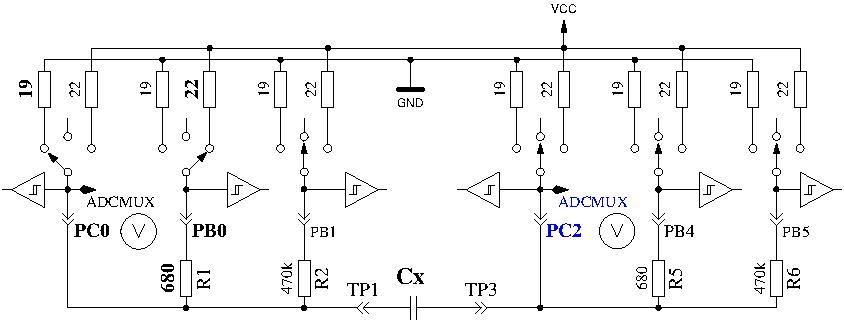
\includegraphics[]{../FIG/Cap_residV.pdf}
\caption{Messung der Kondensator-Restspannung bei Ladebeginn}
\label{fig:CapResidV}
\end{figure}

Abbildung~\ref{pic:c229} zeigt das Laden und Entladen eines \(229\mu F\) großen Kondensators.
Das flache Dach der Messkurve bis zum Entladebeginn ist durch die Messzeit und Berechnungszeit des ATmega verursacht.
Abbildung~\ref{pic:c5mF} zeigt die gleiche Messung mit einem~\(5mF\)-Kondensator,
beachte wie die Messzeit inklusive Entladung auf ungefähr 1,5 Sekunden angewachsen ist.
Das letzte Beispiel in Abbildung~\ref{pic:c15mF} zeigt die Messung eines \(15mF\)-Kondensators.

\begin{figure}[H]
  \begin{subfigure}[b]{9cm}
    \centering
    \includegraphics[width=9cm]{../PNG/charge_229uF.png}
    \caption{\(229\mu F\)-Kondensator}
    \label{pic:c229}
  \end{subfigure}
  ~
  \begin{subfigure}[b]{9cm}
    \centering
    \includegraphics[width=9cm]{../PNG/charge_5mF.png}
    \caption{\(5mF\)-Kondensator}
    \label{pic:c5mF}
  \end{subfigure}
  \caption{Laden und Entladen von großen Kondensatoren für die Messung}
\end{figure}

\begin{figure}[H]
  \centering
    \includegraphics[]{../PNG/charge_15mF.png}
  \caption{Laden und Entladen eines \(15mF\)-Kondensators für die Messung}
  \label{pic:c15mF}
\end{figure}

Nach dieser Kondensatormessung wird die Selbstentladung des Kondensators untersucht, indem der
Spannungsverlust in einer der Ladezeit proportionalen Zeit untersucht wird.
Der gemessene Kapazitätswert wird entsprechend korrigiert. Ein Test mit einer Parallelschaltung von
einem \(68\mu F\)-Kondensator mit einem \(2,2k\Omega\)-Widerstand zeigt die
Wirksamkeit der Methode. Der ermittelte Kapazitätswert ohne den Widerstand beträgt \(66,5\mu F\),
mit dem parallelen \(2,2k\Omega\) Widerstand wird ein Kapazitätswert von \(65,3\mu F\) gemessen.
Zum Vergleich möchte ich die entsprechenden Ergebnisse mit einem Peaktech 3315 Multimeter angeben.
Ohne den Widerstand wird eine Kapazität von \(68,2\mu F\) gemessen, mit dem parallelen \(2,2k\Omega\)
Widerstand wird aber \(192\mu F\) mit dem Multimeter gemessen.

\subsection{Messen von kleinen Kapazitäten}
Wenn der erste \(10ms\) Ladepuls den Kondensator zu hoch aufgeladen hat, wird eine andere Messtechnik benutzt.
Der ATmega-Mikrocontroller hat einen eingebauten 16-Bit-Zähler, der bei voller Taktfrequenz (\(1MHz\) oder \(8MHz\)) arbeiten kann.
Diese Zähler hat auch die Fähigkeit aufgrund eines externen Ereignisses den Zählerstand zu sichern.
Dieses Ereignis kann auch das Ausgangs-Signal des Komparators sein.
Der Komparator kann mit jedem ADC-Eingangspin und der Spannungsreferenz (Band Gap Reference) arbeiten.
Das Schaltbild~\ref{fig:comparat} zeigt ein vereinfachtes Diagram der Messsituation.
So entlade ich den Kondensator, bereite den Komparator für den richtigen Pin-Eingang vor, starte den Zähler bei 0 und
starte sofort das Laden des Kondensators.
Dabei ist eine Seite des Kondensators mit GND, die andere Seite über den \(470k\Omega\)-Widerstand mit VCC verbunden.
Nun prüfe ich in einer Programm-Schleife, ob der Zähler ein Überlauf-Ereignis (overflow) oder ein
 externes Ereignis (input capture) meldet.
Die Überlauf-Ereignisse zähle ich, bis ich ein externes Ereignis feststelle.
In diesem Fall halte ich den Zähler an und prüfe, ob ich noch einen zusätzlichen Überlauf zählen muss, 
weil der Zähler nicht mit dem externen Ereignis (input capture) angehalten werden kann.


Der Zählerstand des externen Ereignisses bildet zusammen mit dem Überlaufzähler die Gesamtzeit, aus der die
Kapazität mit einem Faktor bestimmt wird.
Die aktuelle Software kann eine Tabelle mit der theoretischen Abhängigkeit der Ladezeit in Bezug auf die gemessene
Komparator-Spannung berücksichtigen.
Die Tabelle besitzt Einträge in Schritten von \(50mV\), die Ergebnisse werden entsprechend der aktuellen Referenz-Spannung interpoliert.
Diese Tabelle wird nur mit der Makefile Option WITH\_AUTO\_REF aktiviert.
Vom Kapazitätswert ziehe ich eine experimentell herausgefundene vordefinierte Konstante oder eine im Selbsttest
herausgefundene Konstante ab, um den Messwerte-Offset zu beseitigen.
Ich weiß nicht, ob die vordefinierte Konstante für andere Leiterplatten angepasst werden muss.
Mit einem Selbsttest bei gesetzter AUTO\_CAL-Option wird diese Anpassung automatisch erledigt.

Ich habe bemerkt, dass die Referenz-Spannung meistens etwas zu klein gemessen wird,
 deshalb kann man einen Zusatz mit der Makefile Option REF\_C\_KORR angeben.
Nach der Kalibration mit der AUTO\_CAL-Option ist der REF\_C\_KORR-Wert nur ein Zusatz zu der automatisch
gefundenen Differenz zwischen geladener Kondensator-Spannung und der internen Referenz-Spannung.
Die gemessene Referenz-Spannung wird dann mit dem Korrekturwert (in mV) korrigiert (addiert).
Wenn die Option WITH\_AUTO\_REF nicht benutzt wird, werden die Referenz-Spannungen entsprechend den Angaben in den
Datenblättern ~\cite{ATmega8}~\cite{ATmega168} der ATmega8, ATmega168 und ATmega328 berücksichtigt.
Eine Beispielmessung von diesem Typ ist in Abbildung~\ref{pic:c22uF} dargestellt.
Die Messzeit für den \(22\mu F\)-Kondensator beträgt ungefähr \(2,6s\) weil der \(470k\Omega\)-Widerstand für das Laden benutzt wird.
Aber das Entladen geht in diesem Fall viel schneller als das Laden.

\begin{figure}[H]
\centering
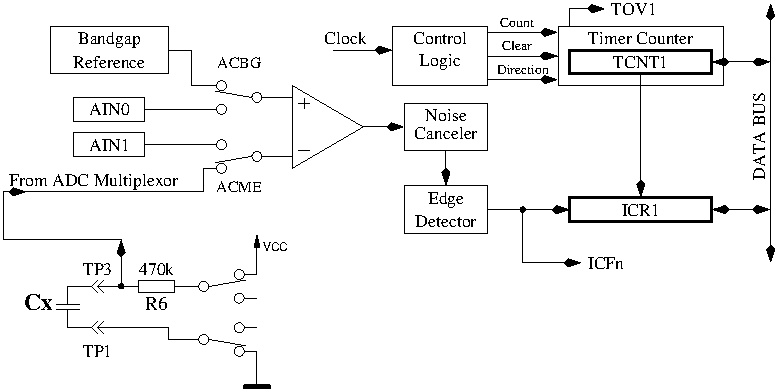
\includegraphics[]{../FIG/Comparat.pdf}
\caption{Messung kleiner Kapazitätswerte mit dem Komparator}
\label{fig:comparat}
\end{figure}

\begin{figure}[H]
  \centering
    \includegraphics[]{../PNG/charge_22uF.png}
  \caption{Laden und Entladen eines \(22\mu F\)-Kondensators für die Messung}
  \label{pic:c22uF}
\end{figure}


Im Prinzip kann diese Technik auch mit dem \(680\Omega\)-Widerstand benutzt werden,
aber weil während dem Komparatorbetrieb der ADC nicht benutzt werden kann, besteht keine
Möglichkeit die Ladespannung zu beobachten bis der Komparator angehalten wird.
Wenn eine unentdeckte Diode mit dem Kondensator parallelgeschaltet ist, kann der Ladestrom
von der Diode aufgenommen werden (Schwellspannung) und die Referenz-Spannung würde nie erreicht.
Dieser Konzeptfehler wird mit der Methode vermieden, die in der aktuellen Software für große Kondensatoren in Kapitel~\ref{sec:bigcap}
verwendet wird.

\subsection{Messen sehr kleiner Kapazitäten mit der Samplingmethode}
Der Funkamateur Pieter-Tjerk (PA3FWM) hat für die Messung sehr kleiner Kapazitäten (\textless~100pF) mit hoher Auflösung
die Fähigkeiten des Testers um die Sampling ADC Methode erweitert.
Die Wandlungsdauer des ADC reicht eigentlich nicht aus, um schnelle Vorgänge abtasten zu können.
Bei der Abtastung der Spannung wird das Eingangssignal aber zu einer exakt festgelegten Zeit abgetastet,
der Sample und Hold Zeit (SH). Der ADC braucht für eine komplette Wandlung 13 Takte, wobei der
ADC Takt durch Teilung des Prozessortaktes durch 128 oder 64 gewonnen wird.
Die Abtastung des Spannungswertes findet immer genau bei ADC-Takt Nummer 1.5 statt. 
Wenn nun das abzutastende Spannungssignal immer wieder neu erzeugt werden kann,
kann man durch Verschiebung der Abtastzeit das komplette Signal mit dem Raster der Verschiebung abtasten.
Eine normale ADC-Wandlung dauert bei 8 MHz Prozessortakt 13x64 = 832 Taktzyklen. 
Wenn das Signal nun mit einem 831 Takte Zyklus wiederholt wird, würde die ununterbrochene ADC-Wandlung (Freilauf-Modus)
das Signal bei jeder fortlaufenden Wandlung einen Prozessortakt später abtasten.
Mit dieser Methode muß dafür gesorgt werden, daß die erste ADC-Abtastung des Signals zu der
gewünschten Startzeit beginnt. Die Zeiten der fortlaufenden ADC Werte verschieben sich dann jeweils um einen
Prozessortakt relativ zum neu erzeugten Signal. Wenn die Wiederholung des Signals gut gelingt, entspricht 
das aus vielen Signalwiederholungen zusammengesetzte Signal dann dem ADC Signal, das mit Prozessortakt (8 MHz) 
abgetastet und gewandelt würde.
Die Abbildung~\ref{fig:sampling} zeigt das Prinzip der Abtastung mit einem zehnmal wiederholten Signal
um daraus 10 Abtastwerte (SH0 - SH9) zu gewinnen.
Für den wirklichen Fall ist die relative Zeitverschiebung der aufeinanderfolgenden Abtastungen 
viel geringer als dargestellt.

\begin{figure}[H]
\centering
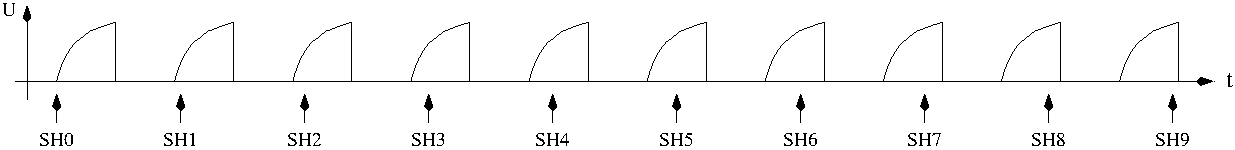
\includegraphics[width=18cm]{../FIG/sampling.pdf}
\caption{Abtasten eines Spannungsverlaufs mit der Samplingmethode}
\label{fig:sampling}
\end{figure}

Eine Schwierigkeit für die genaue Festlegung der ersten Abtastzeit ergibt sich dadurch, daß der
Teiler für die Takterzeugung des ADC nur mit einem externen Signal neu gestartet werden kann.
Bei Start des ADC aus dem Programm läuft der Teiler einfach weiter.
Die Einhaltung der exakten Start- und Perioden-Zeiten ist nur mit einer Funktion in Assemblersprache möglich,
da es auf jeden Prozessortakt ankommt.
Bei der Abtastung der Ladekurve von kleinen Kondensatoren mit der Sampling Methode hat sich auch gezeigt,
daß die Zeitkonstante während der Abtastperiode nicht konstant bleibt. Das hat Pieter-Tjerk bei einem
Vortrag auf der 60. UKW-Tagung in Weinheim dargestellt. Der Kondensator von etwa 10~pF,
der die Spannung für die ADC-Wandlung festhält,
wird zur SH-Zeit für die Wandlung abgekoppelt und etwa zwei ADC-Takte später wieder angekoppelt.
Daneben gibt es einen halben ADC-Takt vorher noch eine kleine Unregelmäßigkeit in den Daten, die wahrscheinlich
vom Schalter des Multiplexors verursacht wird. Beide Störungen werden von der Software berücksichtigt.
Die Sampling Software kann 255 Werte digitalisieren, wobei für die Abtastung der Ladekurven auch der Mittelwert
über 32 Digitalisierungen gebildet werden kann.
Damit können Störeinflüsse etwas geringer gehalten werden.
Die Software kann sowohl einen Ladevorgang als auch einen Entladevorgang vermessen. Weil bei der
Messung der Sperrschichtkapazität einer Diode beide Vorgänge gemessen werden, wird die Kalibration der
Nullkapazität für beide Richtungen und alle Pinkombinationen durchgeführt. 
Mit der Messung der Kapazitäten beim Lade- und Entlade-Vorgang kann die Abhängigkeit der Sperrschichtkapazität
von der Spannung gezeigt werden, da der Ladevorgang die Kapazität in der Nähe von 0V und der Entladevorgang
die Kapazitär in der Nähe von 5V misst. Ein normaler Kondensator sollte bei so kleinen Spannungen keine
Kapazitätsdifferenz zeigen. Hier wird deshalb die Kapazität nur beim Ladevorgang gemessen.
Pieter-Tjerk hat die Funktion für 16~MHz Betrieb optimiert. Hierbei wird eine Auflösung von 0.01~pF erreicht.
Bei 8~MHz Betrieb läuft der ADC-Wandler für die Sampling Methode mit der halben Taktrate, damit die 
vorhin erwähnten Störeinflüsse an den gleichen Datenpositionen liegen.
Der Auflösungsverlust durch den 8~MHz Betrieb spielt wohl meistens keine Rolle und auch die Meßzeit
bleibt im erträglichen Rahmen.

\subsection{Messen des äquivalenten Serienwiderstandes ESR}
Der ESR \cite{ESR} stellt zum Beispiel ein Maß für die Alterung von Elektrolyt-Kondensatoren dar.
Die Abbildung~\ref{fig:Cap_equiv} zeigt ein Ersatzschaltbild eines Kondensators.
Der Widerstand \(Rp\) stellt den Isolationswiderstand des Kondensators dar, \(ESL\) die äquivalente
Serieninduktivität und der Widerstand \(ESR\) stellt den äquivalenten Serienwiderstand dar.

\begin{figure}[H]
  \centering
    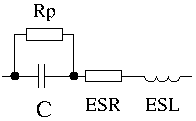
\includegraphics[]{../FIG/Cap_equiv.pdf}
  \caption{Ersatzschaltbild eines Kondensators}
  \label{fig:Cap_equiv}
\end{figure}

Es ist in Datenblättern üblich, den ESR gemessen bei einer Frequenz von \(100kHz\) und
einer Temperatur von \(20{\degree}C\) anzugeben.
Die Abbildungen \ref{fig:Cap_FC_data} und \ref{fig:Cap_FR_data} zeigen die vom Hersteller Panasonic 
angegebenen ESR-Werte für die Elektrolytkondensatoren verschiedener Betriebs-Spannungen für die FC- und die ,,low ESR'' FR-Reihe.
Beide Serien sind für eine maximale Temperatur von \(105{\degree}C\) ausgelegt.
Die Abbildung \ref{fig:Cap_FC_FR_data} stellt die angegebenen Daten beider Serien bei einer zulässigen Betriebsspannung
von \(25V\) dar. Wenn in der Baureihe verschiedene Ausführungen mit gleicher Kapazität und Spannung zur Verfügung stehen,
werden die Daten mit dem niedrigsten ESR dargestellt.
Bei Elektrolytkondensatoren sind sowohl der ESR-Wert als auch die Kapazität relativ stark von der Betriebstemperatur
abhängig.

\begin{figure}[H]
  \centering
    \includegraphics[width=14cm]{../GNU/Cap_FC_dataGE.pdf}
  \caption{ESR-Werte aus dem Panasonic Datenblatt der Serie FC}
  \label{fig:Cap_FC_data}
\end{figure}

\begin{figure}[H]
  \centering
    \includegraphics[width=14cm]{../GNU/Cap_FR_dataGE.pdf}
  \caption{ESR-Werte aus dem Panasonic Datenblatt der Serie FR}
  \label{fig:Cap_FR_data}
\end{figure}

\begin{figure}[H]
  \centering
    \includegraphics[width=14cm]{../GNU/Cap_FC_FR_dataGE.pdf}
  \caption{Vergleich der ESR-Werte der Serie FC mit der Serie FR}
  \label{fig:Cap_FC_FR_data}
\end{figure}

Eine Messung bei \(100kHz\) ist mit der Hardware des ATmega nicht ohne weiteres möglich, da weder der ADC
eine direkte Abtastung einer so hohen Eingangsfrequenz zuläßt, noch ein \(100kHz\) Signal bei der vorhandenen Schaltung zur
Verfügung steht. 
Als nächstes werden hier zwei Methoden für die Bestimmung des ESR vorgestellt, die mit der vohandenen
Schaltung auskommen. 
Beide Methoden verwenden für die Messung ein rechteckförmiges Messsignal, sodass die Ergebnisse nie
exakt mit den Angaben übereinstimmen können, die bei einem sinusförmigen Signal gemessen werden.
Bei der ersten Methode liegen die Ergebnisse nahe bei den ESR-Werten, die bei \(1kHz\) ermittelt werden.
Die zweite Methode hat aber den Vorteil, dass der Nullwert mit kurzgeschlossenen Testpins ermittelt werden kann
und dass zusätzlich der ermittelte ESR sich dem bei \(10kHz\) Messfrequenz gemessenen Wert nähert.
Ich habe derzeit keine Idee für eine Messmethode, die einen direkt zu der \(100kHz\)-Messung einen 
vergleichbaren ESR-Wert liefern kann.

Die folgende Tabelle \ref{tab:capESR} soll die Abhängigkeit des ESR von der Frequenz zeigen.
Außer dem \(47\mu F\) Kondensator sind alle Kondensatoren aus der Baureihe FC von Panasonic.
Die Referenzwerte wurden mit einem Peaktech 2170 LCR-Messgerät ermittelt.
Alle TransistorTester-Resultate in dieser Tabelle wurden mit der im Unterkapitel \ref{sec:ESR2} 
beschriebenen Methode 2 gemessen.
Bei großen Kapazitätswerten macht die ebenfalls vorhandene Induktivität ESL das Messen bei höheren Frequenzen 
wie \(100kHz\) schwierig.


\begin{table}[H]
  \begin{center}
    \begin{tabular}{| l | c | c | c | c | c |}
   \hline
            & Datenblatt & PeakTech  & Peaktech & PeakTech & Transistor- \\
Kondensator & 100 kHz    & 100 kHz   & 10 kHz   & 1 kHz    & tester  \\
    \hline
    \hline
1uF / 50V    & 2.4       & 1.27      & 1.75     & 4.31     &  2.1 \\
    \hline
2.2uF / 50V  & 1.8       & 1.07      & 1.34     & 2.76     &  1.6 \\
    \hline
4.7uF / 50V  & 1.3       & 1.19      & 1.40     & 2.37     &  1.5 \\
    \hline
4.7uF / 50V  & 1.3       & 1.19      & 1.40     & 2.37     &  1.5 \\
    \hline
10uF / 50V   & 1.3       & 1.26      & 1.45     & 2.05     &  1.5 \\
    \hline
22uF / 10V   & 2.0       & 1.52      & 1.76     & 2.24     &  1.9 \\
    \hline
47uF / 63V   & ?         & 0.46      & 0.50     & 0.63     &  0.52 \\
    \hline
    \end{tabular}
  \end{center}
  \caption{ESR-Werte verschiedener Elektrolyt-Kondensatoren}
  \label{tab:capESR} 
\end{table}


\subsection{Messen des äquivalenten Serienwiderstandes ESR, Methode 1}
Bei Kondensatoren mit mehr als \(0,45\mu F\) wird versucht, den Serienwiderstand von Kondensatoren zu messen.
Bei mehr als \(3,6\mu F\) wird dazu die normale Taktrate von \(125kHz\) für den Analog-Digital Wandler benutzt.
Bei kleineren Kapazitäten wird eine erhöhte Taktrate von \(500kHz\) benutzt, um die Messung zu beschleunigen.
Die Genauigkeit der ADC-Ergebnisse wird bei der höheren Taktrate zwar schlechter, aber die größeren ESR-Werte
bei kleineren Kondensatoren mildern die Auswirkung dieses Genauigkeitsverlusts ab. 
Andererseits ist sonst nach diesem Verfahren keine ESR-Messung für Kondensatoren unter \(1,8\mu F\) möglich.

Genau genommen ist der ESR eines Kondensators abhängig von der Betriebsfrequenz und der Temperatur.
Üblicherweise wird der mit einem sinusförmigen Signal bei \(100kHz\) gemessene Wert in Datenblättern angegeben.
Bei dieser Frequenz kann der ATmega ohne externe Beschaltung keine Messung durchführen.
Das nachfolgend beschriebene Verfahren erreicht bei der normalen ADC-Taktrate nur eine Messfrequenz von unter \(640Hz\)
 mit näherungsweise rechteckigem Signal. Bei \(500 kHz\) ADC-Taktrate wird etwa \(2400Hz\) Messfrequenz erreicht.
Um den äquivalenten Serienwiderstand zu bestimmen,
 wird der Kondensator zuerst in einer Richtung geladen und an beiden Anschlüssen die Spannung mit der internen
Referenzspannung (\(1,1V\)) gemessen.
Nach der Messung wird der Ladestrom abgeschaltet und die Spannung am Kondensator ohne den
Ladestrom gemessen. Wenn die Spannung am Kondensator ohne Ladestrom weniger als \(3mV\) beträgt, wird
diese Messfolge wiederholt.
Die Abbildung~\ref{fig:Cap_esr} zeigt die entsprechenden Schaltungen.

\begin{figure}[H]
 \centering
 \begin{overpic}[width=15cm]{../FIG/Cap_esr.pdf}
   \color{black}
   \put(28,85){\makebox(0,0)[cb]{Spannungsmessung mit Ladestrom}}
   \put(28,40){\makebox(0,0)[cb]{Spannungsmessung ohne Strom}}
  \end{overpic}
  \caption{Schaltbild der ESR-Messung eines Kondensators}
  \label{fig:Cap_esr}
\end{figure}

Die Differenz der Spannung am Kondensator mit und ohne Strom ist ein Maß für den internen Widerstand des Kondensators.
Die zu erwartende Spannungsdifferenz ist allerdings so gering, dass mit einer Messung kein brauchbares Ergebnis erzielt
werden kann.
Aus diesem Grund wird danach der Strom umgekehrt und die Messung in der anderen Richtung wiederholt.
Die gesamte Mess-Sequenz wird 128 Mal durchgeführt und die Ergebnisse der Spannungsmessungen addiert.
Danach hat man drei Spannungssummen, die Spannung \(Ulp\) am Minuspol des Kondensators mit Strom, die Spannung \(Uhp\) am
Pluspol des Kondensators mit Strom und die Spannung \(Uc\) am Pluspol des Kondensators ohne Strom.
Die Spannungssumme am Minuspol des Kondensators repräsentiert den Spannungsabfall bei einem mittleren
Ladestrom am Port-Ausgangswiderstand \(Rport\). Aus der Differenz der Spannungssumme am Pluspol und Minuspol des Kondensators
hat man ein Maß für die Spannung am Kondensator mit Ladestrom \(Udiff = Uhp - Ulp\).
Die Differenz \(Uesr = Udiff - Uc\) soll jetzt den Spannungsabfall bei mittlerem Ladestrom am internen Widerstand des Kondensators
repräsentieren.
Der Widerstandswert wird aus dem Verhältnis dieser Spannung \(Uesr\) zu der Spannung \(Ulp\) skaliert mit dem
bekannten Widerstandwert des Port-Ausgangs \(Rport\). Dabei wird so skaliert, dass eine Widerstandauflösung von
\(0,01 \Omega\) erreicht wird \(Resr = \frac{Uesr \cdot 10 \cdot Rport}{Ulp}\).
Die Abbildung~\ref{pic:esr4} zeigt den Ausschnitt des Spannungsverlaufs eines \(4,2\mu F\) Kondensators
 während der ESR-Messung. Dem Kondensator wurde ein \(6,8 \Omega\) Widerstand in Serie geschaltet, um den ESR-Einfluß
zu verdeutlichen. Der kleine Spannungseinbruch nach dem Ladevorgang des Kondensators wird von der Software ausgewertet.
Der größere Spannungseinbruch bei der Messung gegen GND kommt durch den Einfluß des Port-Ausgangswiderstands von etwa \(20\Omega\) zustande.
Das Ergebnis der ESR-Messung ist in diesem Fall \(7,5 \Omega\), ohne den \(6,8 \Omega\) Widerstand sind es \(0,56\Omega\).
Die Abbildung~\ref{pic:esr2} zeigt die gleiche Messung mit höherer Messfrequenz bei einem \(2,2\mu F\) Elko mit einem ESR von \(6.5\Omega\).


\begin{figure}[H]
  \begin{subfigure}[b]{9cm}
    \centering
    \includegraphics[width=9cm]{../PNG/ESR_4uF.png}
    \caption{Ein Pin gegen GND gemessen}
  \end{subfigure}
  ~
  \begin{subfigure}[b]{9cm}
    \centering
    \includegraphics[width=9cm]{../PNG/ESR4uF6R8.png}
    \caption{Von Pin zu Pin gemessen}
  \end{subfigure}
  \caption{Spannungsverlauf eines \(4,2\mu F\) Kondensators während der ESR-Messung}
  \label{pic:esr4}
\end{figure}

\begin{figure}[H]
  \begin{subfigure}[b]{9cm}
    \centering
    \includegraphics[width=9cm]{../PNG/ESR_2uF_pin2GND.png}
    \caption{Ein Pin gegen GND gemessen}
  \end{subfigure}
  ~
  \begin{subfigure}[b]{9cm}
    \centering
    \includegraphics[width=9cm]{../PNG/ESR_2uF_pin2pin.png}
    \caption{Von Pin zu Pin gemessen}
  \end{subfigure}
  \caption{Spannungsverlauf eines \(2,2\mu F\) Kondensators während der ESR-Messung}
  \label{pic:esr2}
\end{figure}

Die Genauigkeit der ESR-Messung ist aus verschiedenen Gründen nicht sehr hoch:
\begin{enumerate}
\item Die Spannungsmessung an den beiden Kondensator-Anschlüssen kann nicht gleichzeitig sondern nur nacheinander durchgeführt werden.
 In der Zwischenzeit hat sich der Ladestrom durch den Ladevorgang des Kondensators geändert.
Dies wird versucht mit einer kapazitätsabhängigen Korrektur der Minuspol-Spannung auszugleichen.
\item Der ADC nimmt den Spannungswert 1,5 Takte nach dem Start des Wandlungsvorgangs. Der Wandelvorgang beginnt mit
der steigenden Flanke des ADC-Taktes, wenn das Startbit gesetzt ist. Wenn der Ladestrom des Kondensators zu früh abgeschaltet wird,
nimmt der ADC die falsche Spannung für die strombehaftete Messung auf. Wird der Ladestrom zu spät abgeschaltet, wird
der Kondensator weiter geladen als es der strombehafteten Messung entspricht.
Dann wird im stromlosen Zustand eine zu hohe Spannung gemessen.
Es ist aber schwierig im Programm den genauen Zeitpunkt für die Stromabschaltung zu treffen.
\item Der Port-Ausgangswiderstand wird bei dieser Messmethode als Referenz benutzt, dessen Widerstandwert
ist aber auch nicht exakt bekannt.
\item Die Auflösung des ADC reicht nicht aus, um eine Widerstandsauflösung von \(0,01\Omega\) zu erreichen.
Für alle Messungen wird die interne Spannungsreferenz (\(1,1V\)) benutzt, um die best mögliche Auflösung zu verwenden.
Zusätzlich wird versucht, den Auflösungs-Mangel durch eine große Zahl von Einzelmessungen abzumildern.
\item Mit der Abfrage des Fertig-Signals der ADC-Wandlung gelingt es nicht exakt, die Schaltzeiten der Port-Ausgänge mit dem
ADC-Takt zu synchronisieren.
\end{enumerate}

Trotz allen Schwierigkeiten scheinen die Ergebnisse brauchbar zu sein, wie die nachfolgende Abbildung \ref{fig:Cesr} zeigt.
Die ESR-Werte eines Bauteils gemessen mit dem Transistortester schwanken stärker als die Messungen des LCR-Meters.
Die Messergebnisse des LCR-Messgerätes wurden bei einer Frequenz von \(1kHz\) gemessen oder für kleine Kapazitäten auf
\(2,4kHz\) interpoliert.
Beim Transistortester muss auf die Qualität der Anschlüsse geachtet werden. Verwendete Anschlusskabel
erhöhen den gemessenen Widerstandswert. Auch die Kontakte von Steckverbindern können die gemessenen
Widerstandwerte erhöhen. Das LCR-Messgerät macht hier wegen den verwendeten Kelvin-Klemmen weniger Probleme.
Bei den Kondensatoren mit einer Kapazität unter \(1\mu F\) war ein \(500nF\) keramischer 
Kondensator (Z5U), alle anderen waren Folien-Kondensatoren. Der einzige Elektrolyt-Kondensator der Messreihe unter \(9\mu F\)  
ist ein \(2,2\mu F\) Kondensator.

\begin{figure}[H]
\centering
 \includegraphics[width=16cm]{../GNU/CesrGE.pdf}
\caption{Messergebnisse der ESR-Messungen mit 15 verschiedenen ATmega}
\label{fig:Cesr}
\end{figure}

\newpage
\subsection{Messen des äquivalenten Serienwiderstandes ESR, Methode 2}
\label{sec:ESR2}
Ab der Softwareversion 1.07k wurde die ESR-Messung auf eine modifizierte Messmethode umgestellt.
Die einzelnen Messschritte sind in Abbildung~\ref{fig:Cap_esr2} gezeigt. Das Besondere an der Methode
ist, dass die Zeit des Stromflusses durch den Kondensator wesentlich gegenüber der Methode 1 verringert wurde.
Der Kondensator wird mit einem Puls der halben Breite negativ vorgeladen und wird dann zyklisch aufgeladen und in der
Gegenrichtung wieder entladen.
Dabei wird der Ladepuls zeitlich so gelegt, dass bei Sample 4 und 8 zur Pulsmitte
die Spannung für den ADC abgegriffen wird (Sample and Hold, 2,5 ADC-Takte nach dem Start).
Ein kompletter Messzyklus wird in Abbildung~\ref{fig:Cap_esr2_timing} gezeigt.
Es werden auch bei dieser Messmethode die Summen der Messergebnisse aus 255 Zyklen ausgewertet,
um eine ausreichende Auflösung zu erreichen.
Eine fortlaufende Aufladung des Kondensators in die eine oder andere Richtung wird durch die kurzen und
gleich langen Auflade- und Entlade-Pulse bei gleicher Beschaltung weitgehend vermieden.
Bei der Messung der Referenzspannung fließt kein Strom durch den Kondensator. Dadurch ist diese Messung
nicht zeitkritisch. Es wird lediglich vorausgesetzt, dass der Kondensator seine Spannung in der
stromlosen Zeit beibehält.

\begin{figure}[H]
  \centering
    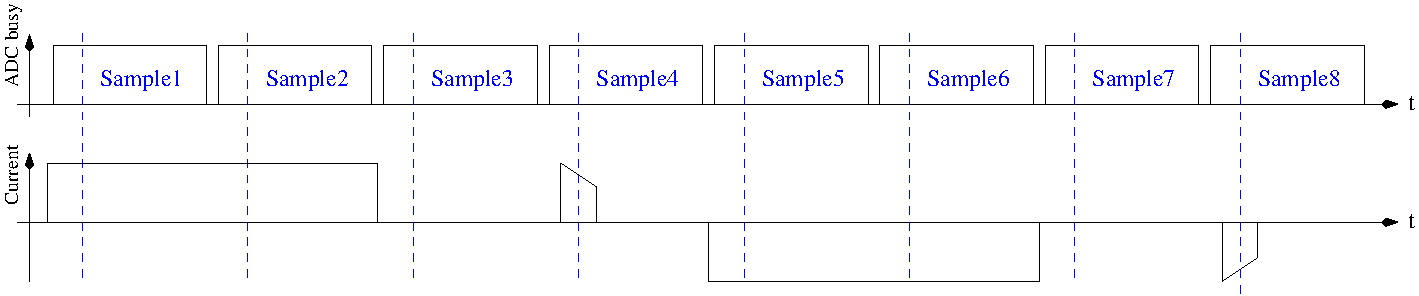
\includegraphics[width=18cm]{../FIG/Cap_esr2_timing.pdf}
  \caption{Zeitlicher Ablauf eines Messzyklus der neuen ESR-Messung}
  \label{fig:Cap_esr2_timing}
\end{figure}

\begin{figure}[H]
 \centering
  \begin{overpic}[width=15cm]{../FIG/Cap_esr2.pdf}
   \color{black}
   \put(20,98){\makebox(0,0)[cb]{Vorwärts Referenzmessung}}
   \put(20,72){\makebox(0,0)[cb]{Vorwärts Spannungsmessung mit Ladestrom}}
   \put(20,47){\makebox(0,0)[cb]{Rückwärts Referenzmessung}}
   \put(20,21){\makebox(0,0)[cb]{Rückwärts Spannungsmessung mit Ladestrom}}
  \end{overpic}
 \caption{Vereinfachte ESR-Messung eines Kondensators}
 \label{fig:Cap_esr2}
\end{figure}


Durch den kürzeren Ladepuls kann nicht nur der ESR von geringeren Kapazitätswerten gemessen werden, sondern
diese Methode kann auch für die Messung kleiner Widerstandswerte benutzt werden, wenn die Widerstände
keine messbare Induktivität besitzen. Dadurch kann die Auflösung bei Widerstandswerten unter \(10\Omega\) auf 
\(0,01\Omega\) gesenkt werden. Daneben kann auch der Nullwiderstand für die Widerstandsmessung als auch
für die ESR-Messung im Selbsttestzweig der Kalibration für alle drei Testpin-Kombinationen bestimmt werden.
Auf solide Steckverbindungen oder Klemmverbindungen sollte für stabile Ergebnisse geachtet werden.
Die Messperiode beträgt etwa \(900\mu s\), was einer Frequenz von etwa \(1,1kHz\) entspricht.
Wegen der Kürze der Ladepulse entspricht das Ergebnis aber eher einer Messung mit \(10kHz\).
Als Beispiel wird die Messung eines \(10\mu F\) Folienkondensators einmal direkt und einmal mit einem
\(2,7\Omega\) Serienwiderstand in Abbildung~\ref{pic:NewEsr10} gezeigt.
Deutlich kann man den Einfluß des zusätzlichen Widerstandes beim Vergleich der beiden Diagramme erkennen.
Hier wird auch verständlich, warum die ADC-Messung in der Mitte des Ladepulses erfolgen muss.
Bei großen Kondensatoren bleibt der Ladestrom des Kondensators hinreichend gut konstant,
sodass bei der zeitlichen Mitte des Ladepulses auch die mittlere Spannung gemessen wird.
Bei keineren Kondensatoren ergibt sich ein deutlicherer Unterschied, der aber mit dem
bekannten Kapazitätswert relativ gut kompensiert werden kann.

\begin{figure}[H]
  \begin{subfigure}[b]{9cm}
    \centering
    \includegraphics[width=9cm]{../PNG/NewEsr10uF0R0.png}
    \caption{ohne Serienwiderstand}
  \end{subfigure}
  ~
  \begin{subfigure}[b]{9cm}
    \centering
    \includegraphics[width=9cm]{../PNG/NewEsr10uF2R7.png}
    \caption{mit \(2,7\Omega\) Serienwiderstand}
  \end{subfigure}
  \caption{Spannungsverlauf eines \(10\mu F\) Kondensators während der neuen ESR-Messung}
  \label{pic:NewEsr10}
\end{figure}

Bei Verwendung von \(27\mu s\) langen Strompulsen kann der ESR von Kondensatoren ab etwa \(180nF\) bestimmt werden.
Um noch kleinere Kondensatoren messen zu können, wurde der Strompuls bei Version 1.11k weiter auf \(8\mu s\) verkleinert.
Die Abbildungen~\ref{pic:NewEsr2} zeigen den Spannungsverlauf an einem \(2,2\mu F\) Kondensator ohne und mit
einem \(2,7\Omega\) Serienwiderstand.

\begin{figure}[H]
  \begin{subfigure}[b]{9cm}
    \centering
    \includegraphics[width=9cm]{../PNG/NewEsr2u2F0R0.png}
    \caption{ohne Serienwiderstand}
  \end{subfigure}
  ~
  \begin{subfigure}[b]{9cm}
    \centering
    \includegraphics[width=9cm]{../PNG/NewEsr2u2F2R7.png}
    \caption{mit \(2,7\Omega\) Serienwiderstand}
  \end{subfigure}
  \caption{Spannungsverlauf eines \(2,2\mu F\) Kondensators während der ESR-Messung mit \(8\mu s\) Ladepulsen}
  \label{pic:NewEsr2}
\end{figure}

Weil in den Abbildungen \ref{pic:NewEsr2} der Zeitpunkt der Spannungsübernahme des ADC nicht zu erkennen ist,
wird in den Abbildungen \ref{pic:NewEsr2zoom} der Ladepuls gedehnt dargestellt. Der Zeitpunkt der Spannungsübernahme
des ADC ist hier etwa in der Bildmitte.

\begin{figure}[H]
  \begin{subfigure}[b]{9cm}
    \centering
    \includegraphics[width=9cm]{../PNG/NewEsr2u2F0R0zoom.png}
    \caption{ohne Serienwiderstand}
  \end{subfigure}
  ~
  \begin{subfigure}[b]{9cm}
    \centering
    \includegraphics[width=9cm]{../PNG/NewEsr2u2F2R7zoom.png}
    \caption{mit \(2,7\Omega\) Serienwiderstand}
  \end{subfigure}
  \caption{Ausschnitt des Spannungsverlaufs eines \(2,2\mu F\) Kondensators während der ESR-Messung mit \(8\mu s\) Ladepulsen}
  \label{pic:NewEsr2zoom}
\end{figure}
 

Die Messergebnisse der neuen ESR-Messmethode sind in Abbildung~\ref{fig:Cesr2} dargestellt.
Die ESR-Werte unterscheiden sich wegen der Frequenzabhängigkeit von den Ergebnissen der Abbildung~\ref{fig:Cesr}.
Die Vergleichswerte des LCR-Messgerätes sind bei \(10kHz\) ermittelt worden.

\begin{figure}[H]
\centering
 \includegraphics[width=16cm]{../GNU/Cesr2GE.pdf}
\caption{Messergebnisse der ESR-Messungen mit 15 veschiedenen ATmega, Methode 2}
\label{fig:Cesr2}
\end{figure}

Eine Messreihe mit Elektrolyt-Kondensatoren verschiedener Größen zeigt die Abbildung \ref{fig:ElcoESR}.
Es werden die Ergebnisse von einem PeakTech 3315 LCR-Messgerät bei verschiedenen Messfrequenzen und die
Ergebnisse des TransistorTesters gegenübergestellt. Die Widerstandswerte sind in diesem Diagram logarithmisch dargestellt.
In allen Fällen liegen die Ergebnisse des TransistorTesters
nahe an den Ergebnissen des LCR-Messgerätes bei \(10kHz\) Messfrequenz. 
Nur der \(500\mu F/3V\) Kondensator war ein älteres Exemplar, alle anderen waren neuwertig.

\begin{figure}[H]
\centering
 \includegraphics[width=16cm]{../GNU/Elco_esrGE.pdf}
\caption{Ergebnisse der ESR-Messungen von verschiedenen Elektrolyt-Kondensatoren}
\label{fig:ElcoESR}
\end{figure}

Da mit der neuen Methode auch Widerstände gemessen werden können, werden in Abbildung~\ref{fig:res_esr} die
Messfehler der Messung von einigen Widerständen unter \(10\Omega\) mit jeweils drei Exemplaren verschiedener
ATmega gezeigt.  

\begin{figure}[H]
\centering
\includegraphics[width=18cm]{../GNU/res_esrGE.pdf}
\caption{Messfehler von Widerständen mit der ESR Messung}
\label{fig:res_esr}
\end{figure}

Ab der Softwareversion 1.12k wurde die Ladepulslänge für die Kondensatoren auf \(2\mu s\) verkürzt, um den ESR Wert bei noch 
geringeren Kapazitätswerten messen zu können. Es kann jetzt der ESR-Wert ab einer Kapazität von \(20nF\) gemessen werden.
Dabei wächst der Meßfehler mit geringer werdender Kapazität an. Der Grund hierfür ist die kleiner werdende Zeitkonstante
der RC-Schaltung, die bei \(20nF\) nur etwa \(14.4\mu s\) beträgt. Dadurch ändert sich die Spannung auch während des
\(2\mu s\) Strompulses deutlich.
Die Software kann den Abtastzeitpunkt nur auf einen Prozessortakt genau wählen. Aber das Eingangsfilter
des ADC hat eine Zeitkonstante von etwa \(0.24\mu s\), die wohl leider von Exemplar zu Exemplar etwas variiert.
Diese Änderung der Filterzeitkonstante kann im Programm nicht berücksichtigt werden.
Hierfür müsste der Abtastzeitpunkt des ADC auf einen Bruchteil der Prozessortaktzeit genau eingestellt werden können.
Mit größer werdenden Kapazitätswerten
des Meßobjektes wächst die Zeitkonstante an und die Spannungsänderung während des Ladepulses wird immer geringer.
Damit hat auch die Variation der Zeitkonstante des ADC-Eingangsfilters immer weniger Einfluß auf die Meßergebnisse.
Die Beispiele in Abbildung~\ref{pic:Cesr_22n} zeigen die Ergebnisse von 10 verschiedenen Testern. Auf der linken Seite
sind Kondensatoren mit höheren ESR-Werten vermessen worden. Da sieht das Ergebnis verglichen mit den
Meßergebnissen des Peaktech 2170 LCR Meßgerätes bei \(10kHz\) und \(100kHz\) noch einigermaßen zufriedenstellend aus.
Auf der rechten Seite sind die Meßwerte von qualitativ guten Kondensatoren mit niedrigen ESR-Werten dargestellt.
Obwohl hier die Grenze des Verfahrens deutlich zu erkennen ist, ist das Ergebnis immer noch besser als gar keine Information.
Es läßt sich in jedem Fall die Qualität eines Kondensators auch bei niedriger Kapazität einschätzen.

\begin{figure}[H]
  \begin{subfigure}[b]{9cm}
    \centering
    \includegraphics[width=9cm]{../GNU/Cesr_22nGE.pdf}
    \caption{höhere ESR Werte}
  \end{subfigure}
  ~
  \begin{subfigure}[b]{9cm}
    \centering
    \includegraphics[width=9cm]{../GNU/Cesr_22n_lowGE.pdf}
    \caption{niedrigere ESR Werte}
  \end{subfigure}
  \caption{ESR-Messungen von Kondensatoren mit niedriger Kapazität}
  \label{pic:Cesr_22n}
\end{figure}
 
Für Prozessoren mit mehr als 16K Flash Speicher wird ab Softwareversion 1.12k für die Hälfte der Einzelmessungen
zusätzlich zum \(680\Omega\) Widerstand der \(470k\Omega\) Widerstand parallel geschaltet, um den Meßstrom geringfügig zu variieren.
Leider ist der zusätzliche Strom sehr gering, so daß die damit erreichte Spannungserhöhung nur wenig zur Änderung
des ADC-Ergebnisses beiträgt.
Die Spannungserhöhung beträgt nur etwa 20\% eines ADC bits mit der internen \(1.1V\) Referenz.
Wünschenswert wäre eine kleine zusätzliche Rauschspannung am ADC Eingang, die zur Änderung der ADC-Einzelwerte führen würde.
Hiermit wäre dann eine statistische Erhöhung der ADC Auflösung durch Mittelwertbildung möglich. 


\subsection{Spannungsverlust nach einem Ladepuls, Vloss}
Beim Messverfahren von großen Kapazitäten wird der Spannungsverlust nach einem Ladepuls im stromlosen Zustand untersucht.
Die erreichte Ladespannung sinkt bei Elektrolyt-Kondensatoren nach kurzer Zeit wieder etwas ab.
Dieser Spannungsverlust kann durch einen parallel geschalteten Widerstand verursacht werden.
Ich nehme an, dass der Spannungsverlust bei Elektrolyt-Kondensatoren durch eine interne Ladungsverteilung nach
dem Ladepuls verursacht wird. Bei einem langsamen Ladevorgang, wie er bei kleineren Kapazitäten mit dem \(470k\Omega\) Widerstand
gemacht wird, ist diese Umverteilung schon während des Ladevorgangs abgeschlossen. Dann tritt kein messbarer Spannungsverlust nach
der Ladung in der betrachteten Zeitspanne auf. Wird der gleiche Elektrolyt-Kondensator aber mit einem
kurzem pulsförmigen Strom geladen, ist hier auch ein Spannungsverlust durch die nachträgliche Umverteilung
der Ladung zu beobachten. Der gleiche Effekt ist in geringerem Umfang auch bei keramischen Kondensatoren zu beobachten. 
Nach den bisherigen Beobachtungen sind Kondensatoren mit mehreren \% Spannungsverlust verdächtig.
Besonders auffällig in Bezug auf den Spannungsverlust sind auch ältere Papierkondensatoren, die auch für andere Messgeräte
eine Herausforderung sind. Dies will ich in folgender Tabelle verdeutlichen.
\vspace{0.5 cm}

\begin{tabular}{| l | c | c | c | c | c | c |}
   \hline
Kondensator & Nenn-      & PeakTech     & Voltcraft & PeakTech & Transistor- \\
Type        & Kapazität  & LCR 2170     & M2650-B   &  3315    & Tester      \\
    \hline
    \hline
Papier     & 4700pF      & 6.75-10.36nF & 8.00nF    &  25.40nF &  10.71nF   \\
           &             &  Q=2.5-32    &           &          &  Vloss=11 \% \\
    \hline
Papier     & 6800pF      & 9.40-11.40nF & 10.41nF   &  23.30nF &  11.65nF  \\
           &             &  Q=5-25      &           &          &  Vloss=5.0 \% \\
    \hline
unbekannt  & 4700pF      & 5.85-6.33nF  & 6.12nF    &  6.90nF  &  6225pF  \\
           &             &  Q=16-87     &           &          &  Vloss=1.7 \% \\
    \hline
Folie      & 7870pF      & 7.86-7.87nF  & 7.95nF    &  7.95nF  &  7872pF  \\
           &             &  Q= \textgreater~1540    &           &          &  Vloss=0 \% \\
    \hline
Papier     & 22000pF     & 37.4-57.5nF  & 52.8nF    &  112nF   &  118.5nF \\
           &             &  Q=2.5-32    &           &          &  Vloss=12 \% \\
    \hline
Folie      & 22600pF     & 22.4-22.5nF  & 22.57nF   & 22.69nF  &  22.54nF \\
           &             & Q= \textgreater~1540     &           &          &  Vloss=0 \% \\
    \hline
Papier     & 100nF       & 144-256nF    & 177nF     &  318nF   &  529.7nF \\
           &             & Q=2.6-28     &           &          &  Vloss=12 \% \\
    \hline
Keramisch  & 100nF       & 97.7-102nF   & 103.7nF   & 103.3nF  &  103.1nF \\
           &             & Q=90-134     &           &          &  Vloss=0.1 \% \\
    \hline
Folie      & 100nF       & 98.0-101nF   & 101.4nF   & 102.2nF  &  101.6nF \\
           &             & Q=58-700     &           &          &  Vloss=0 \% \\
    \hline
\end{tabular}

\vspace{0.5 cm}

In der Tabelle kann man sehen, dass die Kapazität aller Folienkondensatoren mit befriedigender Genauigkeit von allen
Messgeräten bestimmt werden. Die Kapazitäten und die Güten Q des PeakTech LCR-Messgerätes sind Minumum
und Maximum der Messergebnisse im Frequenzbereich \(100Hz\) bis \(100kHz\).
Bei allen Beispielen in der Tabelle ist der Spannungsverlust Vloss des TransistorTesters groß,
wenn die Kondensatoren eine geringe Güte haben. Nur in diesem Fall sind auch große Abweichungen
der gemessenen Kapazität zu beobachten. Damit der Spannungsverlust eines Kondensators vom
Transistortester gemessen werden kann, muss die gemessene Kapazität größer als \(5000pF\) sein.

\subsection{Separate Kapazitäts- und ESR-Messung}
Die separate Kapazitätsmessung mit anschließender ESR-Messung ist nur für ATmega mit genügend Speicher
über den Bediendialog wählbar. Diese Art der Messung ist dafür gedacht, Kondensatoren im eingelöteten
Zustand messen zu können. 
Bitte sorgen Sie dafür, dass alle Kondensatoren auf der Leiterplatte entladen sind, bevor Sie mit den
Messungen beginnen.
Um die Messung im eingebauten Zustand zu ermöglichen, wird dafür gesorgt,
dass die Messspannung möglichst nur knapp über \(300mV\) beträgt.
Außerdem wird für die Messung nur mit dem \(680\Omega\) Widerstand durchgeführt um den Einfluss von
Restströmen der angeschlossenen Bauteilen auf der Leiterplatte gering zu halten.
Um möglichst kleine Kapazitätswerte messen zu können, wird mit einem nur \(200\mu s\) kurzen Ladepuls
begonnen. Wenn die Ladespannung erwarten läßt, dass auch bei einem \(2ms\) langen Ladepuls die Ladespannung
von \(300mV\) nicht überschritten wird, wird danach \(2ms\) lang weitergeladen. Wenn bei sehr großen
Kapazitätswerten auch dann noch kein deutlicher Spannungszuwachs festzustellen ist, wird sogar mit
\(20ms\) langen Ladepulsen weitergeladen. Bei Annäherung der Spannung an die \(300mV\) wird wieder
mit den kürzeren Ladepulsen weitergeladen. Die gesamte Ladezeit wird dabei zusammengezählt und nach
Überschreitung der \(300mV\) die Kapazität aus der geladenen Spannung und der Ladezeit bestimmt.
Mit diesem Verfahren sind Kapazitätswerte von etwas unter \(2\mu F\) messbar. Die Obergrenze der Kapazität
bei dieser Messung beträgt wegen einer Ladezeitbegrenzung auf \(2,5s\) etwa \(50mF\).
Wenn ein Kapazitätswert gemessen wurde, wird danach der ESR-Wert des Kondensators mit dem schon
im Kapitel~\ref{sec:ESR2} beschriebenen Verfahren gemessen.
Die Ergebnisse werden nur kurz angezeigt und danach sofort mit der nächsten Messung begonnen.
Die Messserie wird nach 250 Messungen oder auf Tastendruck abgebrochen und dann zum Bedienmenü zurückgekehrt.

\subsection{Ergebnisse der Kondensator-Messung}
Die Ergebnisse meiner Messungen werden in Abbildung~\ref{fig:mega8cap} für drei ATmega8 dargestellt.
Zusätzlich sind einige Werte der Original-Software mit einem Korrekturfaktor
von 0,88~(\(-12\%\)) dargestellt.
Weitere Ergebnisse von ATmega8-Versionen zeigen die Abbildungen~\ref{fig:mega8Acap} und \ref{fig:mega8Lcap}.
Die Ergebnisse der Messung der gleichen Kondensatoren mit einem ATmega168 werden in Abbildung~\ref{fig:mega168cap} gezeigt.
Die Referenz für die Fehlerberechnung sind die Messwerte eines PeakTech 2170 LCR-Messgerätes, 
 nicht die aufgedruckten Werte der Bauteile.
Die grösseren relativen Messfehler bei großen Kondensatoren liegen zum Teil an der zu hohen Messfrequenz (\(100Hz\)) des
LCR-Messgerätes für große Elektrolytkondensatoren, zum anderen spielt auch die schlechte Güte der
Elektrolytkondensatoren eine Rolle.

\begin{figure}[H]
\centering
\includegraphics[width=16cm]{../GNU/Mega8capGE.pdf}
\caption{Prozentualer Fehler der Kondensator-Messungen mit drei ATmega8}
\label{fig:mega8cap}
\end{figure}

\begin{figure}[H]
  \begin{subfigure}[b]{9cm}
    \centering
    \includegraphics[width=9cm]{../GNU/Mega8AcapGE.pdf}
    \caption{mit drei ATmega8A}
    \label{fig:mega8Acap}
  \end{subfigure}
  ~
  \begin{subfigure}[b]{9cm}
    \centering
    \includegraphics[width=9cm]{../GNU/Mega8LcapGE.pdf}
    \caption{mit drei ATmega8L}
    \label{fig:mega8Lcap}
  \end{subfigure}
  \caption{Prozentualer Kondensator-Messfehler}
\end{figure}

\begin{figure}[H]
\centering
\includegraphics[width=18cm]{../GNU/Mega168capGE.pdf}
\caption{Prozentualer Fehler der Kondensator-Messungen mit dem ATmega168}
\label{fig:mega168cap}
\end{figure}

Wie schwierig es ist, für Kondensatormessungen den richtigen Bezugswert zu finden, soll die Abbildung~\ref{fig:capcompare} zeigen.
Als Bezugswert wurde hier eine beste Schätzung genommen. Die Kurve ,,Multimeter'' zeigt die Abweichungen, die mit einem
Peaktech~3315 Multimeter gemessen wurden.
Die nächste Kurve ,,LCR'' zeigt die Abweichungen, die mit einem Peaktech~2170 LCR-Meter in dem jeweils günstigsten Frequenzbereich gemessen wurden.
Zum Vergleich werden mit der Kurve ,,ATmega168as'' auch noch die Messabweichungen eines ATmega168 bestücktem Transistor-Testers gezeigt.
Ob die gezeigten Fehler aber tatsächliche Messfehler des jeweiligen Gerätes sind, muss bezweifelt werden, da auch die
Schätzung des Kapazitätswert nicht der wirklichen Kapazität entspricht.

\begin{figure}[H]
\centering
\includegraphics[width=18cm]{../GNU/capcompareGE.pdf}
\caption{Vergleich der Kondensator-Messungen mit Multimeter, LCR-Meter und ATmega168}
\label{fig:capcompare}
\end{figure}

Die Abweichungen der Messergebnisse von drei verschiedenen ATmega168 werden in Abbildung~\ref{fig:mega168all} dargestellt.
Hier wurde die Messung des LCR-Meters als Vergleichsbasis genommen.
Entsprechend werden die Messergebnisse von drei verschiedenen ATmega168A in Abbildung~\ref{fig:mega168Aall}, 
von drei verschiedenen ATmega168PA in Abbildung~\ref{fig:mega168PAall} und von drei verschiedenen
ATmega328 in Abbildung~\ref{fig:mega328all} sowie von drei ATmega328P in Abbildung~\ref{fig:mega328Pall} gezeigt.
Hierbei wurde nur der Nullwert der Kapazitätsmessung von \(39pF\) berücksichtigt, alle anderen Korrekturmöglichkeiten wurden
nicht benutzt. Dieser Nullwert beinhaltet schon die \(2-3pF\), die durch die etwa \(12cm\) langen Anschlussleitungen mit den
Klemmen verursacht werden.
Auch das Board-Layout hat Einfluss auf diesen Nullwert. Diesen Nullwert habe ich mit der Boardversion ,,DG2BRS V 5.2.1'' ermittelt.

\begin{figure}[H]
  \begin{subfigure}[b]{9cm}
    \centering
    \includegraphics[width=9cm]{../GNU/Mega168allGE.pdf}
    \caption{drei ATmega168}
    \label{fig:mega168all}
  \end{subfigure}
  ~
  \begin{subfigure}[b]{9cm}
    \centering
    \includegraphics[width=9cm]{../GNU/Mega168AallGE.pdf}
    \caption{drei ATmega168A}
    \label{fig:mega168Aall}
  \end{subfigure}
  \caption{Kondensator-Messfehler, unkalibriert}
\end{figure}

\begin{figure}[H]
\centering
\includegraphics[width=16cm]{../GNU/Mega168PAallGE.pdf}
\caption{Kondensator-Messfehler von drei ATmega168PA, unkalibriert}
\label{fig:mega168PAall}
\end{figure}

\begin{figure}[H]
  \begin{subfigure}[b]{9cm}
    \centering
    \includegraphics[width=9cm]{../GNU/Mega328allGE.pdf}
    \caption{drei ATmega328}
    \label{fig:mega328all}
  \end{subfigure}
  ~
  \begin{subfigure}[b]{9cm}
    \centering
    \includegraphics[width=9cm]{../GNU/Mega328PallGE.pdf}
    \caption{drei ATmega328P}
    \label{fig:mega328Pall}
  \end{subfigure}
  \caption{Kondensator-Messfehler, unkalibriert}
\end{figure}

Zum Erreichen der besten Messgenauigkeit muss die Software an die individuellen Eigenschaften des verwendeten ATmega
angepasst werden. Dazu kann die Korrekturspannung REF\_C\_KORR für den Komparator angegeben werden, der für die Messung der kleinen 
Kapazitäten eingesetzt wird. Eine Korrekturspannung von 1mV führt zu einer Verminderung der Kapazitätsanzeige von etwa 1,1~Promille.
Bei einem automatischen Abgleich ist REF\_C\_KORR  nur ein Offset zu der gemessenen Differenzspannung von geladenem Kondensator
und der internen Referenz.
Für die großen Kapazitäten kann der Promillewert C\_H\_KORR angegeben werden, um den die Messungen
zu groß sind.
Da die großen Kondensatoren meistens Elektrolytkondensatoren mit schlechter Güte sind, ist die Bestimmung
des wahren Kapazitätswertes und damit auch des Messfehlers hier besonders schwierig.

Besonders bei den ATmega168 habe ich bei kleinen Kapazitätswerten einen Messfehler beobachtet, 
der von der Anstiegsgeschwindigkeit der Spannung beim Ladevorgang abhängig ist.
Die Abbildung~\ref{fig:mega168optcap} zeigt die Messabweichung bei Kondensatormessung nur mit der Berücksichtigung des
Nullwertes (168-3-A), mit dem Korrekturfaktor für kleine Kondensatoren REF\_C\_KORR=66 sowie dem Korrekturfaktor für große
Kondensatoren C\_H\_KORR=5 (168-3-B), sowie zusätzlich als Kurve 168-3-C  mit der Berücksichtigung einer Span\-nungs\-an\-stiegs\-kom\-po\-nen\-te 
(COMP\_SLEW1=4000 und COMP\_SLEW2=220) und des Selbst\-ent\-lade\-ver\-hal\-tens der großen Kon\-den\-sa\-toren.
Der Span\-nungs\-an\-stiegs-Kor\-rek\-tur\-faktor berechnet sich nach \(\frac{COMP\_SLEW1}{cval+COMP\_SLEW2} - \frac{COMP\_SLEW1}{COMP\_SLEW2}\),
wobei cval der gemessene Kapazitätswert in pF ist.

\begin{figure}[H]
\centering
\includegraphics[width=16cm]{../GNU/Mega168cap_optGE.pdf}
\caption{Optimierung der Kondensator-Messung eines ATmega168}
\label{fig:mega168optcap}
\end{figure}

\subsection{Automatischer Abgleich der Kondensator-Messung}

Der automatische Abgleich besteht aus zwei Teilen. Der erste Teil besteht darin, einen Nullabgleich der Kondensatormessung durchzuführen.
Dazu wird in der Selbsttest-Routine der Mittelwert der gemessenen Kapazität bei nicht angeschlossenem Kondensator bestimmt.
Es werden die Mittelwerte aus jeweils 8 Messungen für alle 6 Messkombinationen bestimmt.
Nach erfolgreichem Abgleich werden die Korrekturwerte im EEPROM festgehalten und für künftige Messungen verwendet.
Schwieriger ist die Beseitigung der Exemplarstreuungen bei der Messung von Kondensatoren bis etwa \(40\mu F\), wie sie in den 
Abbildungen \ref{fig:mega168all}, \ref{fig:mega168Aall} und \ref{fig:mega168PAall} gezeigt wurden.
Als wesentliche Ursache wurde das unterschiedliche Verhalten (Offset-Spannung) des analogen Komparators herausgefunden.

In Abbildung \ref{fig:CompAdjust} werden die Daten von den neun untersuchten Prozessoren gezeigt.
Die Punkte ,,diff2ref'' zeigen die Spannungsdifferenz, die sich nach dem Laden eines Kondensators mit \(660nF\) zu der
jeweiligen internen Referenzspannung ergibt. Idealerweise wäre diese Spannung immer Null, wenn der analoge
Komparator rechtzeitig das Signal zum Beenden des Ladevorganges gegeben hätte. Die kurze Verwaltungszeit des ATmega
sollte bei der relativ großen Kapazität zu keiner messbaren Spannungserhöhung geführt haben.
Die Punkte ,,CapErr'' zeigen die aus den Abbildungen \ref{fig:mega168all}, \ref{fig:mega168Aall} und \ref{fig:mega168PAall} 
geschätzten Messfehler der einzelnen ATmega-Exemplare in Promille.
Auffällig ist, wie die ,,CapErr'' Punkte den ,,diff2ref'' Punkten folgen.
Deshalb zeigen die Punkte ,,diff'' die Differenz zwischen den jeweiligen ,,CapErr'' und ,,diff2ref'' Punkten.
Für die Korrektur der Kondensatormessung kann also die Differenz der Kondensator-Ladespannung zur internen Referenzspannung
(,,diff2ref'') benutzt werden.
Dabei kann zusätzlich der mittlere Wert der Differenzen zu den ,,CapErr'' Schätzungen (,,diff'') berücksichtigt werden.

Im zweiten Teil der Abgleichprozedur muss also ein Kondensator hoher Güte zwischen Pin~1 und Pin~3 mit einer
Kapazität zwischen \(100nF\) und \(20\mu F\) angeschlossen werden. 
Es sollte ein Folienkondensator, nach Möglichkeit kein keramischer Kondensator und schon gar kein
Elektrolyt-Kondensator sein. Der Kapazitätswert braucht aber für diesen Abgleich nicht genau bekannt zu sein.

\begin{figure}[H]
\centering
\includegraphics[]{../GNU/ComparatorAdjustGE.pdf}
\caption{Daten von neun ATmega168-Prozessoren}
\label{fig:CompAdjust}
\end{figure}

Die Diagramme \ref{fig:mega168cal}, \ref{fig:mega168Acal}, \ref{fig:mega168PAcal},  \ref{fig:mega328cal} und
\ref{fig:mega328Pcal} zeigen die Messergebnisse
der gleichen Prozessoren in einer Standard-Softwarekonfiguration nach der Autokalibration.
Die Prozessoren wurden alle mit der selben Software programmiert, lediglich die Makefile Option ,,PARTNO = '' musste 
wegen dem avrdude-Programm an den unterschiedlichen Prozessortyp (,,m168'', ,,m168p'', ,,m328'' oder ,,m328p'') angepasst werden.
Nach der Programmierung wurde bei jedem ATmega ein
Selbsttest gestartet und bei Test~10 ein Kondensator mit \(330nF\) an Pin~1 und Pin~3 angeschlossen.

\begin{figure}[H]
  \begin{subfigure}[b]{9cm}
    \centering
    \includegraphics[width=9cm]{../GNU/Mega168calGE.pdf}
    \caption{drei ATmega168}
    \label{fig:mega168cal}
  \end{subfigure}
  ~
  \begin{subfigure}[b]{9cm}
    \centering
    \includegraphics[width=9cm]{../GNU/Mega168AcalGE.pdf}
    \caption{drei ATmega168A}
    \label{fig:mega168Acal}
  \end{subfigure}
  \caption{Kondensator-Messfehler, kalibriert}
\end{figure}

\begin{figure}[H]
\centering
\includegraphics[width=16cm]{../GNU/Mega168PAcalGE.pdf}
\caption{Kondensator-Messfehler von drei ATmega168PA, kalibriert}
\label{fig:mega168PAcal}
\end{figure}

\begin{figure}[H]
  \begin{subfigure}[b]{9cm}
    \centering
    \includegraphics[width=9cm]{../GNU/Mega328calGE.pdf}
    \caption{drei ATmega328}
    \label{fig:mega328cal}
  \end{subfigure}
  ~
  \begin{subfigure}[b]{9cm}
    \centering
    \includegraphics[width=9cm]{../GNU/Mega328PcalGE.pdf}
    \caption{drei ATmega328P}
    \label{fig:mega328Pcal}
  \end{subfigure}
  \caption{Kondensator-Messfehler, kalibriert}
\end{figure}

Zuletzt will ich die Wirkung der AUTO\_CAL-Option im Selbsttest noch einmal verdeutlichen.
Die folgende Diagramm \ref{fig:MegaAuto} zeigt die Ergebnisse von drei ATmega-Prozessoren 
mit der grössten Messabweichung noch einmal vor und nach der Kalibration.
Die Punkte mit der Endung ,,unc'' zeigen die Messabweichungen ohne Kalibration.
Die Linien mit der Endung ,,cal'' zeigen die Messabweichungen der gleichen Prozessoren
mit der gleichen Software nach der Kalibration im Selbsttest-Zweig.
Die Ursache der Messabweichungen für große Kondensatoren (\textgreater\(40\mu F\)) ist
noch nicht bekannt. Alle verwendeten Kondensatoren für diese Messreihe waren
Folienkondensatoren oder keramische Kondensatoren (\(56pF\), \(100pF\) und \(3,3nF\)), keine Elkos.

\begin{figure}[H]
\centering
\includegraphics[width=16cm]{../GNU/MegaAutoGE.pdf}
\caption{Kondensator-Messfehler von drei ATmega, vor und nach der Kalibration}
\label{fig:MegaAuto}
\end{figure}

Die Schaltung mit dem ATmega644 oder ATmega1284 sieht einen Kondensator auf der Platine für den Abgleich
vor. Das Diagramm \ref{fig:Mega1284} zeigt die Ergebnisse der Kondensatormessung mit einem ATmega1284,
sowohl mit dem \(100nF\) keramischem Kondensator auf der Platine (1284-int) abgeglichen als auch mit
einem externen \(220nF\) Folien-Kondensator abgeglichen, im Vergleich zu den Ergebnissen eines ATmega328 auf einer
anderen Platine.

\begin{figure}[H]
\centering
\includegraphics[width=16cm]{../GNU/Mega1284GE.pdf}
\caption{Kondensator-Messfehler von einem ATmega1284 im Vergleich zu einem ATmega328}
\label{fig:Mega1284}
\end{figure}
